\chapter{Introducción} 
\label{chap:intro}

\vspace{-0.2cm}
\comments{Veo que sólo existe una tabla: igual no tiene sentido dejar
  el índice de tablas.}
\lsection{Motivación del proyecto}

El derecho a la privacidad en Internet es algo que todo usuario
debería valorar y, por desgracia, \modified{el gran público no le da
  la importancia que debería \cite{book:PrivacyBigDataPublicGood}.}
\comments{Las citas forman parte del texto: se deben escribir como una
  parte más de la frase y, por tanto, estarán antes del signo de
  puntuación.}

No son pocas las noticias que están apareciendo últimamente sobre
empresas como Google relacionadas con la invasión a la
privacidad. Esto, en gran parte, se ha visto incrementado debido a la
llegada de los \textit{smartphones} al mercado(algo relativamente
reciente, hace alrededor de 10 años). El poder llevar en nuestro
bolsillo todo un ordenador tiene el inconveniente de que grandes
empresas como las anteriormente mencionadas pueden tener acceso a
información en tiempo real de nosotros, como por ejemplo a la hora a
la que nos levantamos, la localización de nuestra propia casa e
incluso la ubicación real en todo momento (y sí, de poco sirve
deshabilitar la ubicación por GPS en tu smartphone pues también la
pueden averiguar mediante el inicio de sesión en una red WiFi).
\comments{Te falta alguna referencia, por ejemplo,
  \url{https://techcrunch.com/2017/11/21/android-devices-seen-covertly-sending-location-data-to-google/}. También
es relevante tener en cuenta esto: \url{https://wigle.net/}. Permite
geolocalizar usuarios a través de los SSID. }

Por otro lado está el tema de las redes sociales. Con el auge de
Facebook, Instagram y Twitter, gran parte de la población (en el caso
de Norteamérica, casi dos terceras partes) tiene perfil propio en la
plataforma Facebook \modified{(ver Figura~\ref{fig:norm_Daugman})}.

\begin{figure}[h]
	\centerline{
		\mbox{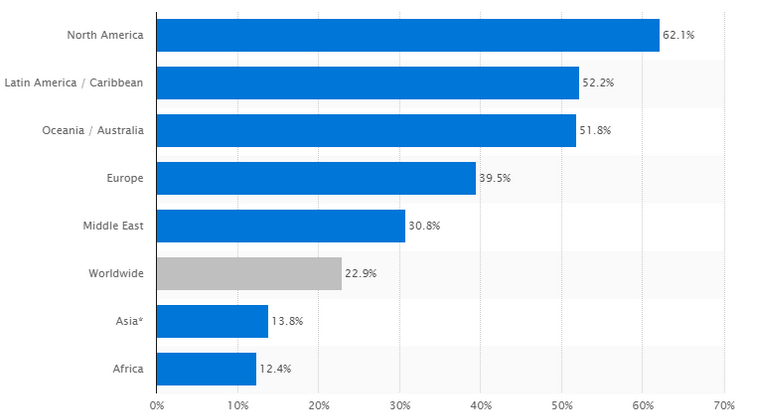
\includegraphics[width=4.00in]{images/sn.png}}
	}
	\caption{Porcentaje de población con perfil en Facebook~\cite{article:FacebookStats} }
	\label{fig:norm_Daugman}
\end{figure}

Esto de por sí no es un dato negativo, el problema viene cuando para realizar un registro en una página (como por ejemplo, la web de un diario), la forma más sencilla es conectando con tu perfil personal de Facebook. Esto causa que, al interaccionar con dicha página(ya sea publicando un comentario, o cualquier tipo de actividad), te arriesgues a que aparezca tu nombre real, con todo lo que ello conlleva. Desde este punto, saber todo acerca de ese usuario es tan sencillo como buscar en Google su nombre completo y entrar a su perfil de Facebook, donde aparecen fotos, su dirección, entre otros(por suerte, esto es algo que desde hace poco podemos evitar~\cite{article:GDPRGoogle} gracias a la recientemente adoptada Ley de Protección de Datos europea, a la cual se hará hincapié en este documento).

En otros casos el iniciar sesión con la cuenta de Google o Facebook sirve para que dichas empresas conozcan mejor tus gustos y hobbies, para así ofrecerte publicidad a medida. 

La motivación de este proyecto reside tanto en un estudio de diversas tecnologías para proteger la privacidad de un usuario mediante el anonimato como en identificar un conjunto de técnicas que suponen una amenaza para nuestra privacidad.
 
Parte de la motivación también reside mi interés en el ámbito de la seguridad informática. Es un tema de suma importancia (algo que puede apreciarse en la creciente demanda de expertos en ciberseguridad hoy en día~\cite{article:expCiberseguridad}) y además sirve para poner en práctica metodologías y lenguajes estudiados en el grado. 

En definitiva, el proyecto  abarca un software modular compuesto de varias herramientas funcionales por sí mismas y donde además el requisito principal es la seguridad del sistema(\textit{security-by-design}~\cite{paper:secbydesign}), y sobre todo que dicho sistema respete la privacidad del usuario (\textit{privacy-by-design}~\cite{paper:privacybydesign} ~\cite{cavoukian2009privacy}). Además, este requisito pasará a ser obligatorio a partir de que entre en vigor la ya mencionada GDPR, por lo que las empresas desarrolladoras de software deberán tener en cuenta la privacidad de los datos de cada usuario en las fases de diseño de todos los proyectos.


\lsection{Objetivos y enfoque}

Principalmente se pretenden lograr dos objetivos fundamentales en este proyecto.

El primero es el de hacernos conocedores más a fondo de las diferentes vías a la hora de anonimizarnos en Internet, las variadas herramientas que pretenden conseguir este objetivo (así como las que pretenden identificar a un usuario), las diferentes nociones del término privacidad~\cite{article:danezis2010}\dots En conclusión, realizar una investigación exhaustiva sobre la privacidad y los caminos para asegurarla.

Por otro lado, y quizá el objetivo más importante, es el de poner en práctica los conocimientos adquiridos en la investigación anteriormente dicha. En este caso se ha diseñado, desarrollado y probado una herramienta con numerosas y diversas funciones, cuyo principal propósito es el de garantizarnos una experiencia lo más anónima posible en todo momento.


\lsection{Metodología y plan de trabajo}

Este documento se organiza de la siguiente manera:
\begin{itemize}
	\item Estado  del  Arte: El segundo capítulo explica todos y cada uno de los conceptos de los que trata este proyecto, es decir, el término privacidad, anonimato y la importancia de los mismos hoy en día. Además, se mostrarán ejemplos de herramientas y metodologías para anonimizarse. 
	\item Análisis: El capítulo tres consta de la serie de requisitos, definidos  según  los objetivos  deseados  en  las  aplicaciones  finales  y  delimitados  por  el  alcance  del proyecto.La funcionalidad de la herramienta desarrollada se resume tanto en el catálogo de requisitos como de casos de uso.
	\item Diseño: Este capítulo trata con detalle la fase de diseño, teniendo en cuenta la estructura de la aplicación y el flujo de navegación de la misma 
	\item Desarrollo: En el quinto capítulo se encuentra explicado el método de desarrollo, las librerías utilizadas, los lenguajes en los que está programada la herramienta, las características Software del equipo de desarrollo y el porqué de dicha elección.
	\item Integración, pruebas y resultados: Aquí se tratan las pruebas unitarias realizadas, así como los resultados de las mismas y cómo se han integrado todos los módulos en la aplicación final.
	\item Conclusiones/Trabajo  futuro: Por último, en este capítulo resumimos las conclusiones de la aplicación y el futuro trabajo que se requeriría para que la herramienta continúe creciendo.
\end{itemize}

\newpage \thispagestyle{empty} % Página vacía 